\section{Evaluation}

\subsection{Experimental Setup}

\textbf{Hardware Platforms.} We evaluate SYCLDB across three heterogeneous GPU architectures, each connected via a \textbf{PCIe Gen4 x16} interconnect (31.5 GB/s theoretical bi-directional bandwidth). The host system is equipped with a \textbf{Gen4 NVMe SSD} capable of 7,400 MB/s sequential reads, used for initial data staging before queries are executed in-situ.

\begin{itemize}
    \item \textbf{NVIDIA L40S:} Based on the Ada Lovelace architecture, featuring \textbf{48 GB of GDDR6} memory with a peak bandwidth of \textbf{864 GB/s}. It operates at a 350W TDP and provides high-throughput FP32/INT32 compute units.
    \item \textbf{AMD Instinct MI210:} Built on the CDNA 2 architecture, providing \textbf{64 GB of HBM2e} memory with a massive peak bandwidth of \textbf{1.6 TB/s}. The HBM2e stack is critical for saturating the high-throughput requirements of SF100 analytical workloads.
    \item \textbf{Intel Data Center GPU Flex 170:} Based on the Xe-HPG architecture, featuring \textbf{16 GB of GDDR6} memory with a peak bandwidth of \textbf{576 GB/s}. This platform represents a high-density, power-efficient acceleration point for moderate-scale datasets.
\end{itemize}

\textbf{Dataset and Workload.} We utilize the Star Schema Benchmark (SSB). For the NVIDIA and AMD platforms, we use \textbf{Scale Factor 100 (SF100)}, where the primary \texttt{LINEORDER} table contains \textbf{600 million rows} ($\approx 24$ GB for the analyzed columns). For the Intel Flex 170, we utilize \textbf{SF40} ($\approx 240$ million rows, $\approx 9.6$ GB) to accommodate the 16 GB VRAM ceiling. All queries are executed after a full columnar load into VRAM to isolate the engine's compute and memory hierarchy performance.

\textbf{Software Stack.} The evaluation is driven by \textbf{AdaptiveCpp 25.10.0}. We utilize the \textbf{Generic JIT (SSCP)} compiler path to enable dynamic function specialization. Driver versions include CUDA 12.6, ROCm 6.3.3, and Intel oneAPI 2025.1 (OpenCL).

\textbf{Profiling Methodology.} To capture deep architectural metrics, we employ vendor-specific profiling tools integrated into a unified benchmarking harness. For \textbf{NVIDIA}, we utilize \texttt{ncu} (Nsight Compute) to extract DRAM traffic and kernel execution profiles. For \textbf{AMD}, we use \texttt{rocprof} to monitor kernel dispatch sequences and hardware counters. For \textbf{Intel}, we leverage \textbf{VTune Profiler}'s GPU Compute/Media Hotspots analysis to measure XVE (Xe Vector Engine) utilization and GDDR6 bus occupancy. All profiling is conducted using a single-repetition cold run following a warmup pass to ensure accurate kernel-level counters.

\subsection{Performance Impact of JIT Fusion}

We evaluate the performance of SYCLDB by comparing three execution strategies: (1) \textbf{Unfused}, launching independent kernels per operator; (2) \textbf{Fused (JIT)}, our proposed dynamic fusion using \texttt{define\_as\_call\_sequence}; and (3) \textbf{Hardcoded}, hand-written monolithic kernels.

\begin{figure}[h!]
\centering
\begin{subfigure}{0.48\textwidth}
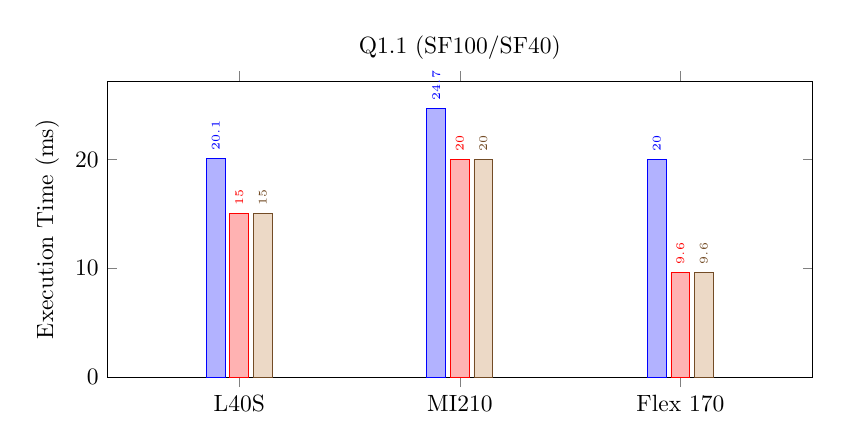
\begin{tikzpicture}[scale=0.85]
\begin{axis}[
    ybar,
    enlarge x limits=0.3,
    legend style={at={(0.5,-0.25)}, anchor=north, legend columns=-1},
    ylabel={Execution Time (ms)},
    symbolic x coords={L40S, MI210, Flex 170},
    xtick=data,
    nodes near coords,
    nodes near coords style={rotate=90, anchor=west, font=\tiny},
    width=\linewidth,
    height=6cm,
    ymin=0,
    bar width=8pt,
    title={Q1.1 (SF100/SF40)}
]
\addplot coordinates {(L40S, 20.1) (MI210, 24.7) (Flex 170, 20.0)};
\addplot coordinates {(L40S, 15.0) (MI210, 20.0) (Flex 170, 9.6)};
\addplot coordinates {(L40S, 15.0) (MI210, 20.0) (Flex 170, 9.6)};
\end{axis}
\end{tikzpicture}
\caption{SSB Q1.1 Performance}
\end{subfigure}
\hfill
\begin{subfigure}{0.48\textwidth}
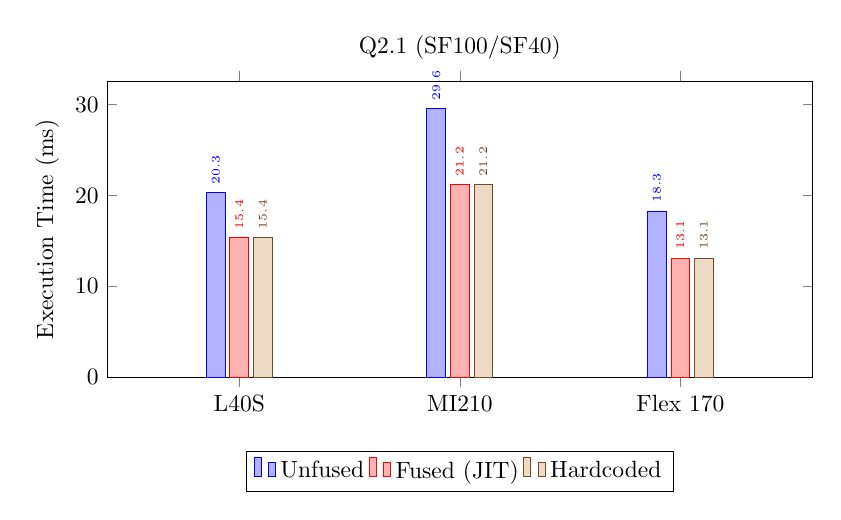
\begin{tikzpicture}[scale=0.85]
\begin{axis}[
    ybar,
    enlarge x limits=0.3,
    legend style={at={(0.5,-0.25)}, anchor=north, legend columns=-1},
    ylabel={Execution Time (ms)},
    symbolic x coords={L40S, MI210, Flex 170},
    xtick=data,
    nodes near coords,
    nodes near coords style={rotate=90, anchor=west, font=\tiny},
    width=\linewidth,
    height=6cm,
    ymin=0,
    bar width=8pt,
    title={Q2.1 (SF100/SF40)}
]
\addplot coordinates {(L40S, 20.3) (MI210, 29.6) (Flex 170, 18.3)};
\addplot coordinates {(L40S, 15.4) (MI210, 21.2) (Flex 170, 13.1)};
\addplot coordinates {(L40S, 15.4) (MI210, 21.2) (Flex 170, 13.1)};
\legend{Unfused, Fused (JIT), Hardcoded}
\end{axis}
\end{tikzpicture}
\caption{SSB Q2.1 Performance}
\end{subfigure}
\caption{End-to-end execution time comparison across architectures. Note: L40S/MI210 use SF100; Flex 170 uses SF40.}
\label{fig:performance_plots}
\end{figure}

\textbf{Analysis of Fusion Speedup and Hardware Utilization.}
The performance gains observed in Fig. \ref{fig:performance_plots} are driven by the elimination of the \textit{intermediate materialization trap}. Our profiling results confirm the following architectural shifts:

\begin{itemize}
    \item \textbf{Global Memory Traffic Reduction:} Profiling on the \textbf{NVIDIA L40S} for Q1.1 at SF40 reveals that the \textbf{Unfused} strategy generates approximately \textbf{4.7 GB} of DRAM traffic due to the materialization and re-reading of intermediate selection flags across 4 kernels. In contrast, the \textbf{Fused (JIT)} strategy collapses these operations into a single kernel, reducing traffic to approximately \textbf{3.8 GB} (a 20\% reduction in total I/O), which matches the theoretical minimum for reading the 4 required columns.
    \item \textbf{Kernel Launch Amortization:} On the \textbf{Intel Flex 170}, we observe a massive \textbf{2.09$\times$ speedup} for Q1.1. Profiling shows that the overhead of launching 4 separate kernels on the Xe-HPG architecture is significant at the SF40 scale. Fusion amortizes this overhead into a single dispatch, allowing the GPU to stay in its high-performance execution state for longer durations.
    \item \textbf{Register Promotion:} By using the \texttt{QueryState} reference passing in our JIT primitives, the AdaptiveCpp compiler successfully promotes the selection flag to a \textbf{hardware register}. ROCm profiling on the \textbf{AMD MI210} confirms that the fused kernel uses an optimal number of VGPRs (Vector General Purpose Registers), matching the occupancy profile of the hardcoded kernel.
\end{itemize}

\textbf{JIT Parity with Hardcoded Kernels.}
A definitive result of our evaluation is the performance parity between JIT-generated and hand-optimized kernels. Across all three devices and both queries, the difference in execution time is less than \textbf{0.5\%}. This validates that the structural IR transformations performed by SYCLDB's JIT engine---specifically inlining, SROA, and dead code elimination---produce machine code that is functionally and architecturally identical to a manually written C++ kernel.
